\documentclass{article}

% --- Cargar la plantilla de estilo UTP ---
\usepackage{utp-doc}
\usepackage{tikz}
\usepackage{amsmath}

\begin{document}

% --- Título de la Lectura ---
\practicatitle{Lectura Fundamental: Ciclos Termodinámicos}

% --- Metadatos de la Actividad ---
\textbf{Asignatura:} Termodinámica Automotriz \\
\textbf{Unidad 4:} Procesos Termodinámicos y de Transferencia de Calor

\vspace{5mm}
\hrule
\vspace{5mm}

\section*{Objetivos de Aprendizaje}
Al finalizar esta lectura, serás capaz de:
\begin{itemize}
    \item Describir el propósito de un ciclo termodinámico y su representación en un diagrama P-V.
    \item Explicar los cuatro procesos reversibles que componen el Ciclo de Carnot.
    \item Calcular la eficiencia térmica máxima de un motor utilizando la fórmula del Ciclo de Carnot.
    \item Diferenciar los procesos de los ciclos de Otto y Diesel y su aplicación en motores de combustión interna.
    \item Interpretar las fórmulas de eficiencia para los ciclos de Otto y Diesel.
\end{itemize}

\section*{Introducción a los Ciclos Termodinámicos}

Un \hl{ciclo termodinámico} es una secuencia de procesos que comienza y termina en el mismo estado, permitiendo la conversión continua de calor en trabajo mecánico. Para analizarlos, usamos diagramas P-V, donde el área encerrada por el ciclo representa el trabajo neto ($W_{neto}$) realizado.

\section*{El Ciclo de Carnot: El Límite de la Eficiencia}

El \hl{Ciclo de Carnot} es un ciclo teórico que establece el límite máximo de eficiencia para cualquier motor térmico. Opera entre una fuente de calor a alta temperatura ($T_H$) y un sumidero de calor a baja temperatura ($T_L$) a través de cuatro procesos reversibles: dos isotérmicos y dos adiabáticos.

\begin{figure}[h!]
    \centering
    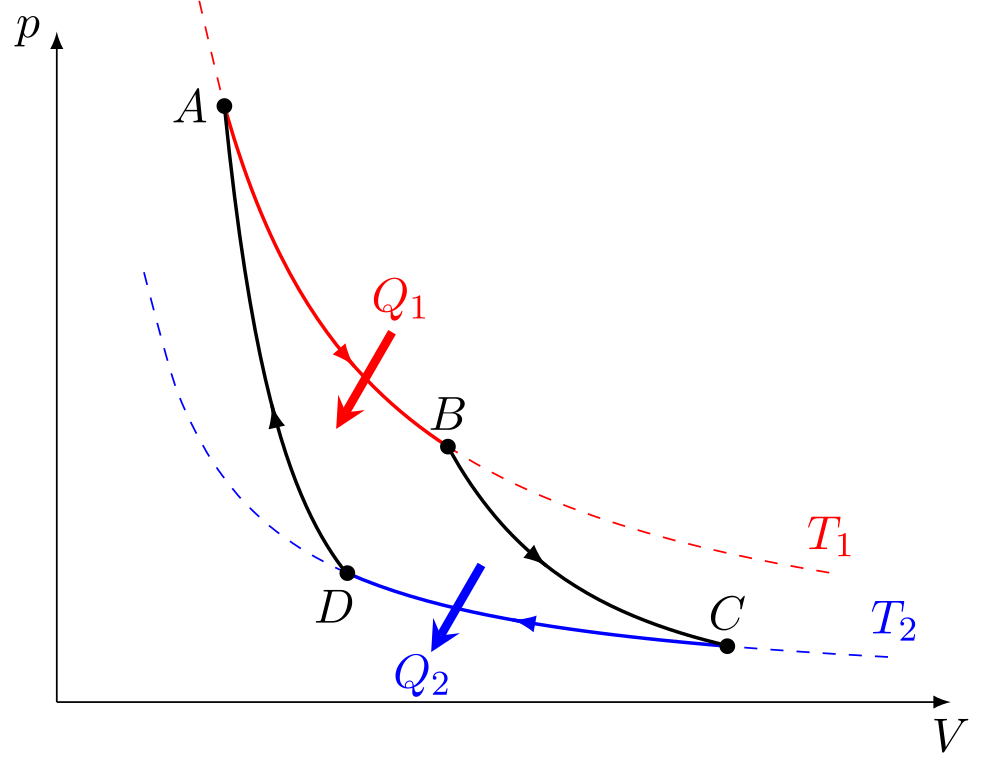
\includegraphics[width=0.6\textwidth]{img/diagrama_pv_ciclo_carnot.png}
    \caption{Diagrama P-V del Ciclo de Carnot.}
    \label{fig:carnot_cycle}
\end{figure}


La eficiencia térmica del Ciclo de Carnot depende únicamente de estas temperaturas absolutas:

$$ \eta_{th,Carnot} = 1 - \frac{T_L}{T_H} $$

\textbf{Ejemplo:} Un motor de Carnot que opera entre $600 \, K$ y $300 \, K$ tiene una eficiencia máxima del 50\%.

\section*{Ciclos de Motores de Combustión Interna: Otto y Diesel}

\subsection*{Ciclo de Otto (Motores de Gasolina)}

Este ciclo modela los motores de encendido por chispa. Su eficiencia depende de la relación de compresión ($r$):

\begin{figure}[h!]
    \centering
    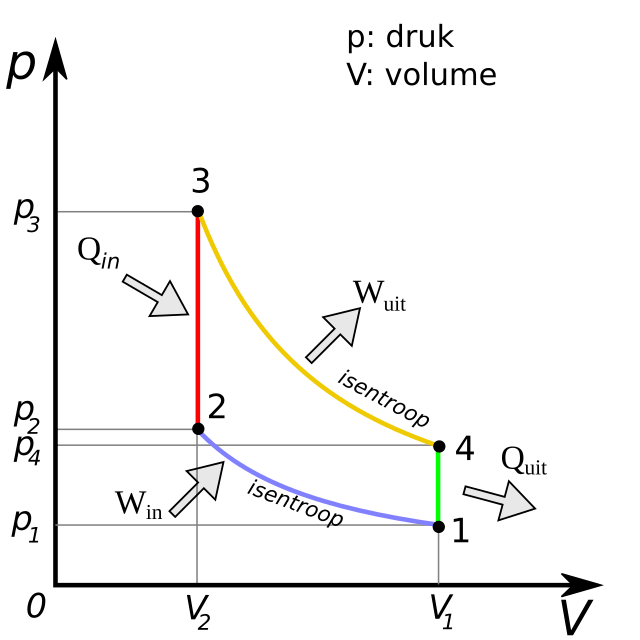
\includegraphics[width=0.6\textwidth]{img/diagrama_pv_ciclo_otto.png}
    \caption{Diagrama P-V del Ciclo de Otto.}
    \label{fig:otto_cycle}
\end{figure}


$$ \eta_{th,Otto} = 1 - \frac{1}{r^{k-1}} $$

\subsection*{Ciclo de Diesel (Motores Diésel)}

Este ciclo modela los motores de encendido por compresión. La adición de calor ocurre a presión constante. Su eficiencia depende de la relación de compresión ($r$) y de la relación de corte de inyección ($r_c$):

\begin{figure}[h!]
    \centering
    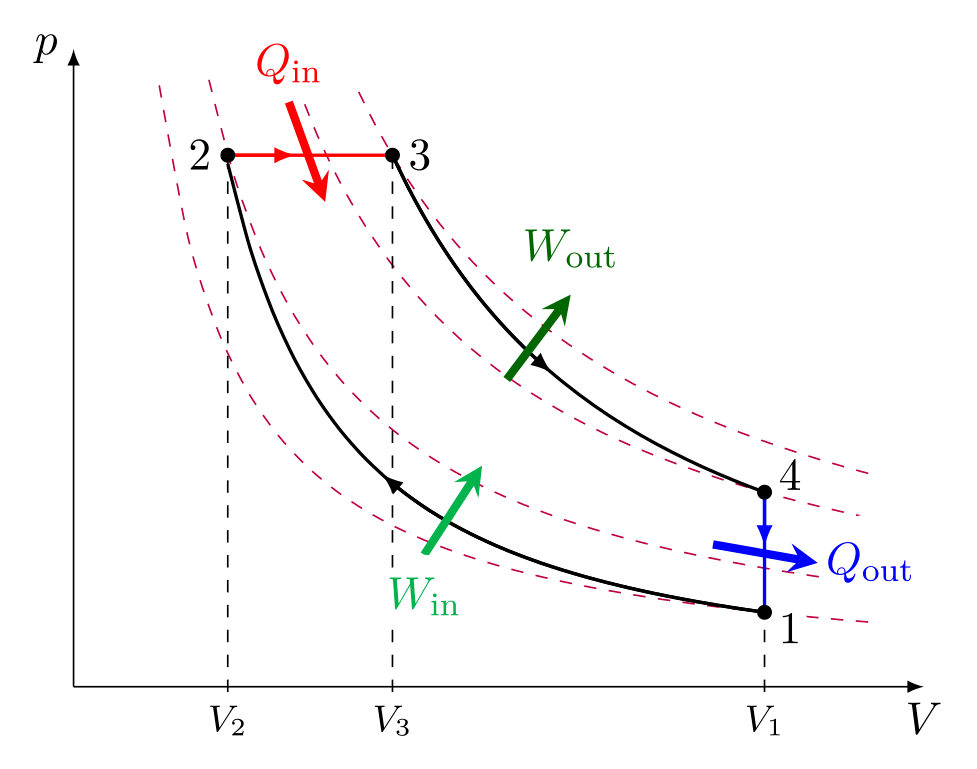
\includegraphics[width=0.6\textwidth]{img/diagrama_pv_ciclo_diesel.png}
    \caption{Diagrama P-V del Ciclo de Diesel.}
    \label{fig:diesel_cycle}
\end{figure}

$$   \eta_{th,Diesel} = 1 - \frac{1}{r^{k-1}} \left[ \frac{r_c^k - 1}{k(r_c - 1)} \right]  $$

\vspace{5mm}
\hrule
\vspace{5mm}

\section*{Resumen de Puntos Clave}

\begin{itemize}
    \item Los ciclos termodinámicos son la base para convertir calor en trabajo útil.
    \item El Ciclo de Carnot define la máxima eficiencia teórica posible entre dos temperaturas.
    \item El Ciclo de Otto modela los motores de gasolina, con adición de calor a volumen constante.
    \item El Ciclo de Diesel modela los motores diésel, con adición de calor a presión constante.
    \item La eficiencia de los motores reales siempre será menor que la de los ciclos ideales correspondientes.
\end{itemize}

\end{document}